\documentclass[10pt]{article}

\usepackage{epsfig}
\usepackage{amsmath}
\usepackage{fullpage}
\usepackage{doublespace}
\setstretch{1.25}

\title{Phased Computation Graphs in the Polyhedral Model}

\author{William Thies, Jasper Lin and Saman Amarasinghe \\
  MIT Laboratory for Computer Science\\
  Cambridge, MA  02139\\ \\
  \texttt{\symbol{`\{}thies, jasperln, saman\symbol{`\}}@lcs.mit.edu}}

% don't include the date
\date{}

\begin{document}

  \maketitle

  \newcommand{\mt}[1]{\mbox{\it #1}}
  \newcommand{\todo}[1]{\framebox{\bf #1}}
  \newcommand{\dep}[0]{Dependence Frontier}                % The full name for the dependence function.
  \newcommand{\DP}[0]{\textsc{Frontier}}                   % Abbrevation for dependence function.
  \newcommand{\DEP}[2]{\DP_{#1 \small{\rightarrow} #2}}    % Math notation for dependence function.

  \begin{abstract}
    Due to the high data rates involved in audio, video, and signal
processing applications, it is imperative to compress the data to
decrease the amount of storage used.  Unfortunately, this implies that
any program operating on the data needs to be wrapped by a
decompression and re-compression stage.  Re-compression can incur
significant computational overhead, while decompression swamps the
application with the original volume of data.

In this paper, we present a program transformation that greatly
accelerates the processing of compressible data.  Given a program that
operates on uncompressed data, we output an equivalent program that
operates directly on the compressed format.  Our transformation
applies to stream programs, a restricted but useful class of
applications with regular communication and computation patterns.  Our
formulation is based on LZ77, a lossless compression algorithm
utilized by ZIP, and immediately applies to simpler formats such as
Apple Animation, Microsoft RLE, and Targa.

We implemented a simple subset of our techniques in the StreamIt
compiler, which emits executable plugins for two popular video editing
tools: MEncoder and Blender.  For common operations such as color
adjustment and video compositing, computing directly on compressed
data offers a speedup roughly proportional to the overall compression
ratio.  For our benchmark suite of 12 videos in Apple Animation
format, speedups range from 1.1x to 471x, with a median of 15x.

  \end{abstract}

  \section{Introduction}


Stream computing represents an increasingly important class of
applications. In streaming codes, there is an abundance of parallelism that
is easier to extract compared to traditional desktop workloads (e.g.,
pointer-based computing). As a result, the extraction of parallelism
in streaming codes does not require heroic efforts, and thus,
processors can deliver higher performance with significantly lower
power costs. This is especially important since
leading microprocessor companies have realized that modern general
purpose architectures are near their  performance limits for  the
amount of power they consume. Thus, the future will place a greater
emphasis on exploiting the properties of streaming workloads in
conventional von~Neumann architectures.

Streaming is a model of computation that uses sequences of data
and computation kernels to expose concurrency and locality for
efficiency~\cite{wss}. In general purpose processors, improving locality 
translates to an effective management of the memory hierarchy at all
levels, including the register file. In this paper, we present a
methodology for compiling streaming codes to general purpose,
cache-based architectures. We first introduce a simple model for
reasoning effectively about the caching behavior of streaming
workloads. This model serves as a foundation for several {\it cache-aware
optimizations} that are geared toward the concomitant increase of instruction
and data {\it temporal locality}. These
optimization lead to significantly better utilization of the memory
system, and as such, they deliver performance gains ranging from 11
to 99\% for our streaming benchmark suite.

The context for our work is StreamIt, an architecture-independent
language that is engineered for streaming
applications~\cite{streamitcc}. It adopts the 
Cyclo-Static Dataflow~\cite{BELP96} model of computation which is a
generalization of Synchronous Dataflow~\cite{LM87-i} (SDF).  
SDF is a popular  model that  is well suited for
streaming codes. In SDF, computation is represented as a graph
consisting of {\it  actors} connected by communication channels; the
actors consume  and produce a constant number  of items from their
input and output  channels every time they execute. SDF is appealing
because it is amenable to static scheduling and optimization. 

From a general purpose architecture's point of view, actors represent
computation kernels, and the communication between actors represents
data buffers that must be streamed to and from the processor. Thus
the size of an actor and the
order of actor executions are critical properties that
impact the performance of the instruction cache. For example, the
compiler must make sure the actor's code size is not
greater than the instruction cache. Furthermore, we must {\it scale}
the execution of the actor so that it runs several times before we move
on to some other actor in the stream 
graph. This serves to $(i)$ amortize the cost of fetching the actor's
instructions into the cache from memory (an expensive operation), $(ii)$
improve the instruction temporal locality, and $(iii)$ improve overall
performance. However, as our cache model will show, we 
cannot arbitrarily scale the execution frequency of an actor. This
is because actors produce data that must be buffered, and therefore,
we must also consider the amount of data an actor produces and
consumes if we are to adequately manage the data cache. This paper is unique
in that it is the first to present a unified optimization methodology
that simultaneously considers instruction and data locality for
mapping streaming computation to cache-based architectures.

In terms of improving the data cache behavior, the compiler schedules
actor firing such that the producer-consumer locality is
preserved. Furthermore,  the compiler may {\it fuse}
together two or more actors to form a coarser grained kernel.
The fusion allows for better register allocation as we can
destroy the arrays used to buffer data between the actors and replace
the corresponding array references with scalars.  It also allows for
various competing implementations for managing the buffers between the
fused actors.  This paper evaluates several implementation
alternatives (for buffer management) and evaluates their performance.

The methodology for fusing actors leverages a distinguishing StreamIt
characteristic, namely, the hierarchical organization of
the stream graph. Furthermore, the algorithm for fusing actors applies
for the various topologies allowed by StreamIt.
It also considers another distinguishing characteristics of StreamIt,
namely the {\tt peek} operation whereby an actor may inspect data
items in its input buffer without consuming them until some future
execution. While peeking is a powerful language feature, it does pose
some challenges to the compiler and the cache optimizations. Peeking
also impacts the choice for the best buffer management strategy, as our
study will show.

%% the comment about p3 and itanium not being embedded architectures
%% is out of the blue! need a better transition.
Cache-aware fusion alone delivers significant performance gains, although our
evaluation shows that fusion with scaling leads to the best
performance on a general purpose, cache-based architecture. For our
experiments, we use two different processors: a superscalar out-of-order
processor, and an in-order VLIW processor. The former is a Pentium~3
whereas the latter is an Itanium~2. While these architectures are not
particularly suited for an embedded system, they do exhibit some
properties that are worthy of investigation. Furthermore, that we can
demonstrate measurable performance gains on real systems is far more
convincing than using a simulation-based environment. We chose the
Pentium~3 processor because it has very few registers in its
instruction set architecture. The Itanium by contrast has a much 
larger and richer repertoire of registers. The two architectures serve
to validate our cache-aware optimizations, in that we expect an
architecture with more register to benefit more from optimization such
as scalar replacement. On average, fusion leads to a 47\% improvement
on the Pentium~3, and 50\% on the Itanium~2.

The two architectures also differ in terms of their memory system
organization. The Itanium is an in-order VLIW processor and does not
tolerate a memory stall as well as its out-of-order
counterpart. Therefore we expect different gains from the scaling
optimization which amortize the long access latencies for instruction
and data caches. On average, scaling leads to a 21\% improvement on
the Itanium~2, and 17\% on the Pentium~3.

While both scaling and fusion lead to modest performance gains, we
must combine the two to deliver the best possible performance. When we
do so, we can further improve the performance of our benchmarks by
53\% on average for the Pentium~3, and 55\% for the Itanium~2.

\subsection{Summary of Contributions}

This paper makes the following contributions:
\begin{itemize}

\item A cache model for stream computing that provides a quantitative
estimate of the caching performance for any sequence of actor
executions.

\item A cache-aware scheduling heuristic that judiciously increases
the multiplicity of actors, improving instruction and data locality
while not exceeding the data cache.

\item A cache-aware partitioning policy that judiciously fuses
adjacent actors into a single component, enabling local optimizations
while not exceeding the instruction cache.

\item An optimized buffer management policy, termed ``copy-shift with
execution scaling'', which out-performs a traditional rotating buffer
in a detailed micro-benchmark analysis.

\item A fully automatic implementation of the above techniques in the
StreamIt compiler.

\item An experimental evaluation across 11 streaming benchmarks,
demonstrating performance improvements of up to 99\%.
\end{itemize}

\subsection{Paper Roadmap}

The remainder of the paper is organized as follows. Section~\ref{sec:streamit}
describes StreamIt and introduces our motivating example.
Section~\ref{sec:cache-model} introduces our cache model for 
reasoning about the performance of a streaming
computation. Section~\ref{sec:cache-opt} describes our cache-aware
optimizations, and Section~\ref{sec:buffer} describes the 
optimization enabled by fusion. Section~\ref{sec:evaluation} describes
our evaluation methodology and present our experimental
analysis. Sections~\ref{sec:related-work}~and~\ref{sec:conclusion}
discuss related work and concludes the paper.

  \section{Related Work}
\label{sec:related}

% BILL

%Signal~\cite{Signal}, 
%Lucid~\cite{Lucid77}, and
%Occam~\cite{Occam}, and Sisal \cite{sisal}.
%Parallel Haskell~\cite{ph}
In addition to StreamIt, there are a number of stream-oriented
languages drawing from domains such as functional, dataflow, CSP and
synchronous programming~\cite{survey97}.  The Brook language is
architecture-independent and focusses on data
parallelism~\cite{brook04}.  Stream kernels are required to be
stateless, though there is special support for reducing streams to a
single value.  Stream\-C/Ker\-nel\-C is lower level than Brook;
kernels written in KernelC are stiched together in StreamC and mapped
to the data-parallel Imagine processor~\cite{imagine03ieee}.  SPUR
adopts a similar decomposition between ``microcode'' stream kernels
and skeleton programs to expose data parallelism~\cite{spur05samos}.
Cg exploits pipeline parallelism and data parallelism, though the
programmer must write algorithms to exactly match the two pipeline
stages of a graphics processor~\cite{cg03}.  Compared to these
languages, StreamIt places more emphasis on exposing task and pipeline
parallelism (all the languages expose data parallelim).
%and on sliding window operations (filters that peek).  
By adopting the synchronous dataflow model of execution~\cite{lee87},
StreamIt focusses on well-structured programs that can be aggressively
optimized.  The implicit infinite loop around programs is also a key
StreamIt characteristic that enables the transformations in this
paper.  Spidle is also a recent stream language that was influenced by
StreamIt~\cite{spidle03}.
%and Lucid Synchrone~\cite{Lucid-Synchrone}.
%Synchronous languages which
%target embedded applications include Esterel~\cite{Esterel},
%Lustre~\cite{Lustre}, and Additional

Liao et al. map Brook to multicore processors by leveraging the affine
partitioning model~\cite{liao06brook}.  While affine partitioning is a
powerful model for parameterized loop-based programs, in StreamIt we
simplify the problem by fully resolving the program structure at
compile time.  This allows us to schedule a single steady state using
flexible, non-affine techniques (e.g., simulated annealing) and to
repeat the found schedule for an indefinite period at runtime.
Gummaraju and Rosenblum map stream programs to a general-purpose
hyperthreaded processor~\cite{gummaraju05micro}.  Such techniques
could be integrated with our spatial partitioning to optimize per-core
performance.  Gu et al. expose data and pipeline parallelism in a
Java-like language and use a compiler analysis to efficiently extract
coarse-grained filter boundaries~\cite{du03sc}.  Ottoni et al. also
extract decoupled threads from sequential code, using hardware-based
software pipelining to distribute the resulting threads across
cores~\cite{ottoni05decoupled}.  By embedding pipeline-parallel
filters in the programming model, we focus on the mapping step.

%%%%%%%%%%%%%%%%%%%%%%%%%%%%%%%%%%%%%%%%%%%%%%%%%%%%%%%%%%%%%%%%%%%%%

Previous work in scheduling computation graphs to parallel targets has
focused on partitioning and scheduling techniques that exploit task
and pipeline parallelism~\cite{SDFSched, SDFSched2,may87communicating,
DAGSched, pipeline-sdf}.  Application of loop-conscious
transformations to coarse-grained dataflow graphs has been
investigated.  Unrolling (or ``unfolding'' in this domain) is employed
for synchronous dataflow (SDF) graphs to reduce the initiation
interval but they do not evaluate mappings to actual
architectures~\cite{unfolding,unfolding2}. Software pipelining
techniques have been applied to SDF graphs onto various embedded and
DSP targets~\cite{bakshi99,chatha-02}, but has required programmer
knowledge of both the application and the architecture. To our
knowledge, none of these systems automatically exploit the combination
of task, data, and pipeline parallelism.  Furthermore, these systems
do not provide a robust end-to-end path for application
parallelization from a high-level, portable programming language.

%% Previous work on instruction-level software pipelining has focused
%% mostly on scheduling machine instructions in a loop via modulo
%% scheduling~\cite{rau81,lam-softpipe}.  The algorithms devised must
%% account for tight resource constraints and complex instruction
%% dependences. Our software-pipelining problem is much less constrained,
%% enabling us to employ a simple greedy heuristic.  

%% Furthermore, a traditional modulo scheduling algorithm is not needed
%% because we have an implicit loop barrier at the end of each
%% steady-state.  ILP compilers for clustered VLIW
%% architectures~\cite{Bulldog,Multiflow,lee98spacetime,qian02} must
%% partition instructions and assign them to clusters as part of the
%% instruction scheduling. Clustering is analogous to our application of
%% filter fusion in our software pipelining algorithm.

  \section{Phased Computation Graphs}
\label{sec:pcg}

\begin{table}[t]
\small
\begin{center}
\begin{tabular}{|c|c|c|c|c|c|} \hline
Model of Computation & Items on Channels & Nodes with & Nodes with & Cyclic Steady & Initialization \\
                     & at Start & Pop $\ne$ Push & Peek $>$ Pop & State Phases & Phases \\
\hline \hline
Synchronous Dataflow~\cite{LM87-i} & X & X & & & \\
\hline
Cyclo-Static Dataflow~\cite{BELP96} & X & X & & X & \\
\hline
Computation Graphs~\cite{KM66} & X & X & X & & \\
\hline
Phased Computation Graphs & X & X & X & X & X \\
\hline
\end{tabular}
\vspace{-6pt}
\caption{\protect\small Models of Computation for Dataflow Graphs.}
\label{tab:models}
\vspace{-12pt}
\end{center}
\end{table}

We introduce the Phased Computation Graph (PCG) as a model of
computation for dataflow languages; specifically, we designed the PCG
as a model for StreamIt~\cite{streamitcc}.  A PCG is a generalization
of the Computation Graph (CG) of Karp and Miller~\cite{KM66} to the
case where each node has both an initial and steady-state execution
epoch, each of which contains a number of {\it phases}.  It is also a
generalization of other popular representations for dataflow graphs,
such as synchronous dataflow (SDF) and cyclo-static dataflow (CSDF)
(see Table~\ref{tab:models}).  Phases are attractive constructs for
the reasons given in describing CSDF in Section~\ref{sec:related};
also, an initial epoch is critical for applications such as a WAV file
decoder that adjusts its parameters based on the data it finds in the
header of the stream.

Formally, a PCG is a directed graph with the following components:
\begin{itemize}

\item Nodes $n_1 \dots n_{m_n}$.

\item Channels $c_1 \dots c_{m_c}$, where each channel is directed
from a given node $n_a$ to a given node $n_b$.

\item A non-negative integer $A(c)$ indicating the number of items
  that are initially present on channel $c$.

\item The number of phases $\mt{num}(n, t)$ that node $n$ exhibits
during epoch $t$.  Here $t$ indicates the type of epoch, which is
either initial ($\mt{init}$) or steady-state ($\mt{steady}$).  For all
$n$, $\mt{num}(n, \mt{init}) \ge 0$ and $\mt{num}(n, \mt{steady}) \ge
1$.

\item Non-negative integers $U(c, t, p)$, $O(c, t, p)$, and $E(c, t,
p)$, which give the number of items pushed, popped, and peeked,
respectively, over channel $c$ during the $p$'th phase of epoch $t$.

\end{itemize}

\subsection{Execution Model}

We give an informal description of the execution semantics of a PCG,
which is an intuitive extension to that of a CG.  An execution
consists of a sequence of atomic {\it firings} of nodes in the graph.
The effect of firing a given node depends on its epoch and its phase,
which are both local states of the node.  At the start of execution,
each node is in phase 0 of the initial epoch, and each channel $c$
contains $A(c)$ items.

Let us consider a node $n$ that is in phase $p$ of epoch $t$.  It is
legal for $n$ to fire if $p \in [0, \mt{num}(n, t)-1]$ and, for each
channel $c_{in}$ directed into $n$, there are at least $E(c_{in}, t,
p)$ items on $c_{in}$.  The effect of this firing is to consume
$O(c_{in}, t, p)$ items from each channel $c_{in}$ directed into $n$;
to produce $U(c_{out}, t, p)$ new items on each channel $c_{out}$
directed out of $n$; and to advance the phase $p$ of $n$ to
$\mt{next}(t, p)$.  In the initial epoch, each phase executes only
once and $\mt{next}(\mt{init}, p) = p + 1$; in the steady-state epoch,
the phases execute cyclically and $\mt{next}(\mt{steady}, p) = (p +
1)~\mt{mod}~\mt{num}(n, t)$.  If a node $n$ is in phase $\mt{num}(n,
\mt{init})$ of the initial epoch, then it transitions to the
steady-state epoch and resets its phase to 0.

From the starting state of the graph, execution proceeds via a
sequence of node firings.  The order of node firings is constrained
only by the conditions given above.

\section{Phased Computation Programs}

The PCG described above is a representation for a graph, treating each
node and channel as a black box.  Here we introduce some notation for
the internals of the nodes, as well as the ordering of items on the
channels.  We refer to the aggregate model as a Phased Computation
Program (PCP).  Before describing a PCP, we will need some additional
notation:
\begin{itemize}

\item We assume that all items passed over channels are drawn from the
same domain of values ${\cal V}$.

\item An array type\footnote{To simplify the presentation, we allow
ourselves a slight abuse of notation by sometimes using arrays instead
of enumerating individual elements.  Our definitions could be expanded
into strict element-wise SARE's without any fundamental change to the
technique.} of length $n$ and element type $\tau$ is denoted by
$\tau[n]$.  Given a two-dimensional array $A$ of type $\tau[n][m]$,
$A[i][*]$ denotes the $m$-element array comprising the $i$'th row of
$A$.

\item $\mt{num\_in}(n)$ (resp. $\mt{num\_out}(n)$) denotes the number of
channels that are directed into (resp. out of) node $n$.

\item $\mt{chan\_in}(n)$ (resp. $\mt{chan\_out}(n)$) denotes the list of
channels that are directed into (resp. out of) node $n$.

\item $\mt{pos\_in}(n, c)$ (resp. $\mt{pos\_out}(n, c)$) denotes the
position of channel $c$ in $\mt{chan\_in}(n)$
(resp. $\mt{chan\_out}(n)$.  That is, $\mt{chan\_out}(n)[\mt{pos\_out(n,
c)}] = c$.

\end{itemize}

A PCP consists of the following:
\begin{itemize}

\item A Phased Computation Graph $G = (\{n_1 \dots n_{m_n}\}, \{c_1
\dots c_{m_c}\}, A, \mt{num}, U, O, E)$ describing the nodes,
channels, and I/O rates of the program (see Section~\ref{sec:pcg}).
Each channel $c = (n_a, n_b)$ is a FIFO queue; $n_a$ pushes items onto
the back of $c$ and $n_b$ consumes items from the front of $c$.

\item The initial values $I(c)$ that are enqueued onto channel $c$ at
the start of execution.  Since there are $A(c)$ initial values on
channel $c$, $I(c)$ has type ${\cal V}[A(c)]$.

%An initialization function $I(c)$ that returns an array of
%length $A(c)$, the elements of which are enqueued onto channel $c$ at
%the start of execution.  The procedure $I(c)$ takes no arguments; its
%signature is $\mt{void} {\small \rightarrow} {\cal V}[A(c)]$.
%
\item A work function $W(n, t, p)$ that represents the computation of
node $n$ in phase $p$ and epoch $t$.  The signature of $W(n, t, p)$ is
$[{\cal V}[E(\mt{chan\_in}(n)[1], t, p)], \dots, {\cal
V}[E(\mt{chan\_in}(n)[\mt{num\_in}(n)], t, p)]]$ $\rightarrow$ \\ $[
{\cal V}[U(\mt{chan\_out}(n)[1], t, p)], \dots, {\cal
V}[U(\mt{chan\_out}(n)[\mt{num\_out}(n)], t, p)]]$.  That is, the
function inputs a list of arrays, each of which corresponds to an
incoming channel $c_{in}$ and contains the $E(c_{in},t,p)$ values that
$n$ reads from $c_{in}$ in a given firing.  The procedure returns a
list of arrays, each of which corresponds to an outgoing channel
$c_{out}$ and contains the $U(c_{out},t,p)$ values that $n$ writes to
$c_{out}$ in a given firing.

\end{itemize}

%The components $I$ and $W$ above are referred to as ``procedures''
%rather than mathematical functions because we expect them to be
%represented as blocks of source code for an actual procedure
%declaration, thereby allowing a straightforward conversion to a PCP
%from a dataflow program.  However, 


  \section{Basic Translation: SDF to SARE}
\label{sec:simple}

In order to familiarize the reader with the basics of our technique,
we present in this section the translation procedure for a simplified
input domain.  The translation rules for the general case can be found
in \todo{Next section??}.

Our basic translation operates on synchronous dataflow graphs with all
of the channels initially empty.  That is, we assume that:
\begin{enumerate}

\item No items appear on the channels at the beginning:  $\forall c, A(c) = 0$.

\item There are no initialization phases: $\forall n, \mt{num}(n, \mt{init}) = 0$.

\item Each node has only one steady-state phase: $\forall n, \mt{num}(n, \mt{steady}) = 1$.

\item There is no peeking: $\forall c, \forall t, \forall p, E(c, t, p) = O(c, t, p)$.

\end{enumerate}

Given these restrictions, we can simplify our notation considerably.
Since we are only concerned with the steady-state epoch and the 0'th
phase of each node, we can omit some arguments to any function that
requires an epoch $t$ or a phase $p$.  For instance, the push and pop
rates of a channel $c$ are now just $U(c)$ and $O(c)$, respectively;
the work function for a node $n$ is simply $W(n)$.

\subsection{Calculating the Steady-State Period}

Let $S(n)$ denote the number of times that node $n$ fires its 0'th
phase for a balanced steady-state execution cycle of the entire
graph. \todo{Say more about this.}

We will use the following helper function.  Given channel $c = (n_a, n_b)$:
\begin{align*}
\mt{Period}(c) \equiv S(n_a) * U(n_a) = S(n_b) * U(n_b)
\end{align*}

\subsection{Generating a SARE}

The SARE will be parameterized by $N$, the number of steady-state
cycles that one wishes to execute in the PCP.

\subsubsection{Variables}

For each channel $c = (n_a, n_b)$, do the following:
\begin{itemize}

\item Introduce variable $\mt{BUF}_c$ with the following domain:
\begin{align*}
{\cal D}_{{BUF}_c} = \{ ~(i,j)~|~0 \le i \le N - 1 ~\wedge~ 0 \le j \le \mt{Period}(c) - 1\}
\end{align*}

\item Introduce variable $\mt{WRITE}_{c}$ with this domain:
\begin{align*}
{\cal D}_{{WRITE}_{c}} = \{~(i,j,k)~|~0 \le i \le N-1 ~\wedge~ 
                                       0 \le j \le S(n_a) - 1 ~\wedge~ 0 \le k \le U(c) - 1\}
\end{align*}

\item Introduce variable $\mt{READ}_{c, p}$ with this domain:
\begin{align*}
{\cal D}_{{READ}_{c}} = \{~(i,j,k)~|~0 \le i \le N-1 ~\wedge~ 
                                      0 \le j \le S(n_b) - 1 ~\wedge~ 
                                      0 \le k \le E(c) - 1\} \\
\end{align*}

\end{itemize}

\subsubsection{Equations}

\noindent For each node $n$, do the following:
\begin{itemize}

\item For each $c \in \mt{chan\_out}(n)$, introduce this equation
(READ to WRITE):
%
\begin{align*}
\forall (i, j, k) \in {\cal D}_{{WRITE}_{c}},~\mt{WRITE}_{c}(i,j,k) = W(n)(\mt{Steady\_Inputs})[\mt{pos\_out}(n, c)][j] \\
\mt{where Steady\_Inputs} = [\mt{READ}_{{chan\_in}(n)[1]}(i, j, *), \dots, 
                             \mt{READ}_{{chan\_in}(n)[\mt{num\_in}(n)]}(i, j, *) ]
\end{align*}
%
\item For each $c \in \mt{chan\_out}(n)$, and for each $q \in
[0,\frac{\mt{Period(c)}}{\mt{U(n)}}-\mt{1}]$,
introduce this equation (WRITE to BUF):
\begin{align*}
\forall (i,j) \in {\cal D}_{SW {\small \rightarrow} SB}(c,q), \\
\mt{BUF}_{c}(i,j) = 
  \mt{WRITE}_{c}(i * \frac{\mt{Period}(c)}{O(c)} + \lfloor \frac{q}{S(n)} \rfloor, q~mod~S(n),
                     j - q * U(c) \\
\mt{where } {\cal D}_{SW {\small \rightarrow} SB}(c,q) = 
  {\cal D}_{{BUF}_{c}} \cap 
  \{ (i,j) | q*U(c) \le j \le (q+1)*U(c) - 1 \}
\end{align*}

% here is the simple, base case of the BUF -> READ function
\item For each $c \in \mt{chan\_in}(n)$, introduce this equation (BUF to
READ):
\begin{align*}
\forall (i,j,k) \in {\cal D}_{{READ}_{c}},
\mt{READ}_{c}(i,j,k) = j*O(n) + k
\end{align*}
\end{itemize}

\begin{figure}[t]
\framebox[6.5in]{
\begin{minipage}{6.5in}
\end{minipage}
}
\end{figure}



  \section{General Translation: CSDP to SARE}
\label{sec:translate}

In this section we give the formal translation of a Cyclo-Static
Dataflow Program to a System of Affine Recurrence Equations.  Again,
the SARE will be parameterized by $N$, the number of steady-state
cycles that one wishes to execute in the CSDP.  The translation will
use the helper functions shown in Figure~\ref{fig:helper}.  We also
make use of the $S(n)$ function giving the number of steady-state
executions of node $n$ (see Section~\ref{sec:balance}).  
%Please refer
%to the Appendix for a concrete illustration of the techniques
%described below.

\begin{figure}[t]
\framebox[6.5in]{
\begin{minipage}{6.3in}
\begin{center}
{\bf Helper Functions}
\end{center}
\begin{itemize}
\item The number of integral points in a one-dimensional domain ${\cal
D}$ is denoted by $|{\cal D}|$.  The sign and absolute value of an
integer $i$ are given by $sign(i)$ and $abs(i)$, respectively.
%
\item $\mt{PartialWrite}(c,t,p) = \sum_{r=0}^{p-1} U(c, t, r)$
%
\item $\mt{TotalWrite}(n,c,t) = \sum_{r=0}^{\mt{num}(n, t)-1} U(c, t, r)$
%
\item $\mt{PartialRead}(c,t,p) = \sum_{r=0}^{p-1} O(c, t, r)$
%
\item $\mt{TotalRead}(n,c,t) =  \sum_{r=0}^{\mt{num}(n, t)-1} O(c, t, r)$
%
\item Given channel $c = (n_a, n_b)$:
\begin{align*}
\mt{Period}(c) \equiv S(n_a) * \mt{TotalWrite}(n_a, c, \mt{steady}) = 
S(n_b) * \mt{TotalRead}(n_b, c, \mt{steady})
\end{align*}
%
\end{itemize}
%
\end{minipage}}
\caption{Helper functions for the PCP to SARE translation.
\protect\label{fig:helper}}
\end{figure}

\begin{figure}[t]
\framebox[6.5in]{
\begin{minipage}{6.3in}
\begin{center}
{\bf Variables}
\end{center}

For each channel $c = (n_a, n_b)$, do the following:
\begin{itemize}

\item Introduce variables $\mt{IBUF}_c$ and $\mt{SBUF}_c$ with the following domains:
\begin{align}
{\cal D}_{{IBUF}_c} = \{~i~|~0 \le i \le A(c) +
\sum_{p=0}^{\mt{num}(n_a, \mt{init})-1} U(c, \mt{init}, p) - 1 \} \\ \nonumber ~ \\
%
{\cal D}_{{SBUF}_c} = \{ ~(i,j)~|~0 \le i \le N - 1 ~\wedge~ 0 \le j \le \mt{Period}(c) - 1\}
\end{align}

\item For each $p \in [0, num(n_a, \mt{init})-1]$, introduce
variable $\mt{IWRITE}_{c, p}$ with this domain:
\begin{align}
{\cal D}_{{IWRITE}_{c, p}} = \{~i~|~0 \le i \le U(c, \mt{init}, p) - 1\}
\end{align}

\item For each $p \in [0, num(n_b, \mt{init})-1]$, introduce
variable $\mt{IREAD}_{c, p}$ with this domain:
\begin{align}
{\cal D}_{{IREAD}_{c, p}} = \{~i~|~0 \le i \le E(c, \mt{init}, p) - 1\}
\end{align}
%
\item For each $p \in [0, num(n_a, \mt{steady})-1]$, introduce
variable $\mt{SWRITE}_{c, p}$ with this domain:
\begin{align}
{\cal D}_{{SWRITE}_{c, p}} = \{~(i,j,k)~|~0 \le i \le N-1 ~\wedge~ 0 \le j \le S(n_a) - 1 ~\wedge~ 0 \le k \le U(c, \mt{steady}, p) - 1\}
\end{align}
%
\item For each $p \in [0, num(n_b, \mt{steady})-1]$, introduce
variable $\mt{SREAD}_{c, p}$ with this domain:
\begin{align}
{\cal D}_{{SREAD}_{c, p}} = \{~(i,j,k)~|~0 \le i \le N-1 ~\wedge~ 0 \le j \le S(n_b) - 1 ~\wedge~ 0 \le k \le E(c, \mt{steady}, p) - 1\}
\end{align}
%
\end{itemize}
%
\end{minipage}}
\caption{Variables for the PCP to SARE translation.
\protect\label{fig:pcptosare1}}
\end{figure}

\begin{figure}[p]
\framebox[6.5in]{
\begin{minipage}{6.3in}
\begin{center}
{\bf Equations (Part 1)}
\end{center}
\noindent For each channel $c = (n_a, n_b)$, introduce the following equations:
\begin{itemize}
%
\item {\bf(I to IBUF)}:
\begin{align}
\forall i \in [0,A(c)-1],~\mt{IBUF}_{c}(i) = I(c)[i]
\label{i2ibuf}
\end{align}

\item {\bf(IWRITE to IBUF)} For each $p \in [0, num(n_a, \mt{init})-1]$:
\begin{align}
\label{iwrite2ibuf}
&\forall i \in [A(c) + \mt{PartialWrite}(c,\mt{init},p),
               A(c) + \mt{PartialWrite}(c,\mt{init},p+1)-1], \\ \nonumber
&~~~~~~\mt{IBUF}_{c}(i) = \mt{IWRITE}_{c, p}(i - A(c) - \mt{PartialWrite}(c,\mt{init},p))\nonumber
\end{align}
%
\item {\bf(IREAD to IWRITE)} For each $c \in \mt{chan\_out}(n)$, and for each $p \in [0,
num(n, \mt{init})-1]$:
%
\begin{align}
\label{iread2iwrite}
&\forall i \in {\cal D}_{{IWRITE}_{c, p}},~\mt{IWRITE}_{c,p}(i) = W(n, \mt{init}, p)(\mt{Init\_Inputs})[\mt{pos\_out}(n, c)][i], \\ \nonumber
&\mt{where Init\_Inputs} = [\mt{IREAD}_{{chan\_in}(n)[1], p}(*), \dots, \mt{IREAD}_{{chan\_in}(n)[\mt{num\_in}(n)], p}(*) ]
\end{align}
%
\item {\bf(SREAD to SWRITE)} For each $c \in \mt{chan\_out}(n)$, and for each $p \in [0,
num(n, \mt{steady})-1]$:
%
\begin{align}
\label{sread2swrite}
&\forall (i, j, k) \in {\cal D}_{{SWRITE}_{c, p}},~\mt{SWRITE}_{c,p}(i,j,k) =\nonumber\\
&~~~~~~W(n, \mt{steady}, p)(\mt{Steady\_Inputs})[\mt{pos\_out}(n, c)][k], \mt{where}\\\nonumber&
\mt{Steady\_Inputs} = [\mt{SREAD}_{{chan\_in}(n)[1], p}(i, j, *), \dots, \mt{SREAD}_{{chan\_in}(n)[\mt{num\_in}(n)], p}(i, j, *) ]
\end{align}
%
\item {\bf(SWRITE to SBUF)} For each $c \in \mt{chan\_out}(n)$, for each $p \in [0,
\mt{num}(n, \mt{steady})-1]$, and for each $q \in [0,S(n)-1]$:
\begin{align}
\label{swrite2sbuf}
&\forall (i,j) \in {\cal D}_{SW {\small \rightarrow} SB}(c,p,q),
\mt{SBUF}_{c}(i,j) = \nonumber\\
&~~~~~~\mt{SWRITE}_{c, p}(i, q,
                     j - \mt{Offset}_{SW {\small \rightarrow} SB}(q,n,c,p)),
\mt{where } \\&{\cal D}_{SW {\small \rightarrow} SB}(c,p,q) = 
  {\cal D}_{{SBUF}_{c}} \cap 
  \{ (i,j) | \mt{Offset}_{SW {\small \rightarrow} SB}(q,n,c,p) \le j
             \le \mt{Offset}_{SW {\small \rightarrow} SB}(q,n,c,p+1) - 1 \} \nonumber\\\nonumber
&\mt{and } \mt{Offset}_{SW {\small \rightarrow} SB}(q,n,c,p') = q*\mt{TotalWrite}(n,c,\mt{steady}) + \mt{PartialWrite}(c,\mt{steady},p'))
\end{align}
%
\item {\bf(IBUF to IREAD)} For each $c \in \mt{chan\_in}(n)$, and for each phase $p \in
[0, \mt{num}(n, \mt{init})-1]$:
\begin{align}
\label{ibuf2iread}
&\forall i \in {\cal D}_{IB {\small \rightarrow} IR}(c,p), 
\mt{IREAD}_{c, p}(i) = \mt{IBUF}_{c}(\mt{PartialRead}(c, \mt{init}, p) + i) \\ \nonumber
&\mt{where }{\cal D}_{IB {\small \rightarrow} IR}(c,p) = 
  \{ i | i \in {\cal D}_{{IREAD}_{c,p}} ~\wedge~ 
         i + \mt{PartialRead}(c, \mt{init}, p) \in {\cal D}_{{IBUF}_{c}} \}
\end{align}
%
\item {\bf(SBUF to IREAD)} For each $c \in \mt{chan\_in}(n)$, for each phase $p \in [0,
\mt{num}(n, \mt{init})-1]$, and for each \\$q \in [0, \lfloor
\frac{\mt{argmax}_{\mt{p}'} \left( \mt{PartialRead}(\mt{c}, \mt{init},
\mt{p}') + \mt{E}(\mt{c}, \mt{init}, \mt{p}') \right)
}{\mt{Period(c)}} \rfloor ]$:
\begin{align}
\label{sbuf2iread}
&\forall i \in {\cal D}_{SB {\small \rightarrow} IR}(c,p), 
\mt{IREAD}_{c,p}(i) = 
    \mt{SBUF}_{c}(q,
      i - \mt{Offset}_{SB {\small \rightarrow} IR}(q,n,c,p)), \mt{where } \\ \nonumber
&{\cal D}_{SB {\small \rightarrow} IR}(c,p) = 
  \{ i | i \in {\cal D}_{{IREAD}_{c,p}} ~\wedge~
         \mt{Offset}_{SB {\small \rightarrow} IR}(q,n,c,p)
         \le i \le
         \mt{Offset}_{SB {\small \rightarrow} IR}(q+1,n,c,p) - 1 \} \\ \nonumber
&\mt{and }\mt{Offset}_{SB {\small \rightarrow} IR}(q',n,c,p) = 
  q' * \mt{Period}(c) + |{\cal D}_{{IBUF}_c}| - \mt{PartialRead}(c,\mt{init},p)
\end{align}
%
\end{itemize}
\end{minipage}}
\caption{Equations for the PCP to SARE translation.
\protect\label{fig:pcptosare2}}
\end{figure}

\begin{figure}[p]
\framebox[6.5in]{
\begin{minipage}{6.3in}
\begin{center}
{\bf Equations (Part 2)}
\end{center}
\noindent For each node $n$, introduce the following equations:
\begin{itemize}
\item {\bf(IBUF to SREAD)} For each $c \in \mt{chan\_in}(n)$, and for each phase $p \in [0,
\mt{num}(n, \mt{steady})-1]$:
\begin{align}
\label{ibuf2sread}
&\forall (i,j,k) \in {\cal D}_{IB {\small \rightarrow} SR}(n,c,p), 
\mt{SREAD}_{c, p}(i,j,k) = 
    \mt{IBUF}_{c}(\mt{ReadIndex}(n,c,p,i,j,k)), \mt{where} \nonumber\\
&\mt{ReadIndex}(n,c,p,i,j,k) = \mt{TotalRead}(n,c,\mt{init})
                + (i*S(n)+j)*\mt{TotalRead}(n,c,\mt{steady}) \\ \nonumber
                &~~~~~~+ \mt{PartialRead}(c, \mt{steady}, p) 
                + k) \\\nonumber
&\mt{and }{\cal D}_{IB {\small \rightarrow} SR}(n,c,p) = 
  \{ (i,j,k) | \mt{ReadIndex}(n,c,p,i,j,k) \in {\cal D}_{{IBUF}_{c}} \}
\end{align}
%
\item {\bf(SBUF to SREAD)} For each $c \in \mt{chan\_in}(n)$, for each phase $p \in [0,
\mt{num}(n, \mt{steady})-1]$, and for each $q \in [0, \lfloor
\frac{\mt{E(c, steady, p)}}{\mt{Period(c)}} \rfloor]$:
% two possible problems: sread has already been written to, or sbuf has already been read from
\begin{align}
\label{sbuf2sread0}
&\forall (i,j,k) \in {{\cal D}\mt{1}}_{SB {\small \rightarrow} SR}(c,p,q),
\mt{SREAD}_{c, p}(i,j,k) = 
    \mt{SBUF}_{c}(i+q+
                  \mt{Int\_Offset}(n,c,p),\nonumber\\ \nonumber
                  &~~~~~~j*\mt{TotalRead}(n,c,\mt{steady}) + 
                    \mt{PartialRead}(c,\mt{steady},p) + k
                   - q * \mt{Period}(c) + \mt{Mod\_Offset}(n,c,p)), \\
&\mt{where }{{\cal D}\mt{1}}_{SB {\small \rightarrow} SR}(c,p,q) = 
  ({\cal D}_{{SREAD}_{c, p}} - \mt{PUSHED}(n,c,p))
                         \cap \\ \nonumber
	&~~~~~~\{ (i,j,k) | q * \mt{Period}(c) - min(0, \mt{Mod\_Offset}(n,c,p))
                                \le k 
                                \le \\ \nonumber
	&~~~~~~~~~~~~min((q+1)*\mt{Period}(c),
         E(c, \mt{steady}, p)) - 1 
         - max(0, \mt{Mod\_Offset}(n,c,p)) \}\\ \nonumber\\
\label{sbuf2sread1}
%\end{align}
%\begin{align}
%
%
&\forall (i,j,k) \in {{\cal D}\mt{2}}_{SB {\small \rightarrow} SR}(c,p,q),
\mt{SREAD}_{c, p}(i,j,k) = \nonumber\\
    &~~~~~~\mt{SBUF}_{c}(i+q+
                  \mt{sign(Offset)} + \mt{Int\_Offset}(n,c,p),
                  j*\mt{TotalRead}(n,c,\mt{steady}) + \\\nonumber
                    &~~~~~~~~~~~~\mt{PartialRead}(c,\mt{steady},p)
		+ k
                   - q * \mt{Period}(c) 
                   - \mt{sign(Offset)} * \mt{Period}(c)
 + \mt{Mod\_Offset}(n,c,p)),\\ \nonumber&
\mt{where }{{\cal D}\mt{2}}_{SB {\small \rightarrow} SR}(c,p,q) = 
  ({\cal D}_{{SREAD}_{c, p}} - \mt{PUSHED}(n,c,p)) \cap \\ \nonumber
                         &~~~~~~( \{ (i,j,k) | q * \mt{Period}(c)
                                \le k 
                                \le min((q+1)*\mt{Period}(c),
                                              E(c, \mt{steady}, p)) - 1 \} - {{\cal D}\mt{1}}_{SB {\small \rightarrow} SR}(c,p,q) )\\ \nonumber\\
\label{sbuf2sread2}
%\end{align}
%\begin{align}
%
%
&\mt{where }\mt{PUSHED}(n,c,p) = {\cal D}_{IB {\small \rightarrow} SR}(n,c,p) \nonumber\\ \nonumber
&\mt{and }\mt{Num\_Pushed}(n,c,p) = 
% this is a dot product of (i,j,k) with something
  (max_{\preceq}\mt{PUSHED}(n,c,p)) \cdot (S(n) * \mt{TotalRead}(n,c,\mt{steady}), \\ \nonumber
                                        &~~~~~~\mt{TotalRead}(n,c,\mt{steady}),
                                        1 ) + \mt{PartialRead}(c, \mt{steady}, p),
\mt{and }\mt{PEEKED}(c,p) = {SB {\small \rightarrow} IR}(c,p) \\ \nonumber
&\mt{and }\mt{Num\_Popped}(c,p) = |\mt{PEEKED}(c,p)| + O(c,\mt{steady},p) - E(c,\mt{steady},p) \\
&\mt{and }\mt{Offset}(n,c,p) = \mt{Num\_Popped}(c,p)-\mt{Num\_Pushed}(n,c,p) \\ \nonumber
&\mt{and }\mt{Int\_Offset}(n,c,p) = \mt{sign(Offset)}*\lfloor \frac{abs(\mt{Offset}(n,c,p))}{\mt{Period}(c)} \rfloor) \\ \nonumber
&\mt{and }\mt{Mod\_Offset}(n,c,p) = \mt{sign(Offset)}*(abs(\mt{Offset}(n,c,p))~\mt{mod}~\mt{Period}(c))
%
\end{align}
%
\end{itemize}
\end{minipage}}
\caption{Equations for the PCP to SARE translation.
\protect\label{fig:pcptosare3}}
\end{figure}

Figure~\ref{fig:csdptosare1} illustrates the variables used for the
translation.  These are very similar to those in the simple case,
except that now there are separate variables for each phase.  The
equations for the translation appear in Figure~\ref{fig:csdptosare3}.
  \section{Precise Event Handling}
In this section we describe how $\sdep$ information can be
incorporated into the semantics of a language feature that provides
precise delivery of control messages in stream programs.  Our goal is
to improve both programmer productivity and performance.

The Synchronous Dataflow (SDF) domain is well-suited for applications
that have regular, high-bandwidth communication patterns.  However, in
realistic streaming applications there are also irregular,
low-bandwidth control messages that are used to adjust parameters in
various parts of the stream.  For example, a downstream actor might
detect a high signal-to-noise ratio and send a message to the
communications frontend to increase the amplification.  Or, an actor
at the top of the stream graph might detect an invalid checksum for a
packet, and send a message downstream to invalidate the effects of
what has been processed.  Other examples of control messages include:
periodic channel characterization; adaptive beamforming; initiating a
handoff ({\it e.g.,} to a new network protocol); marking the end of a
large data segment; and responding to user inputs, environmental
conditions, or exceptional states.

Generally speaking, control messages are sent at infrequent and
irregular intervals; however, once they are generated there might be
tight constraints on their delivery.  For example, the message
invalidating the effects of a given packet has to be delivered exactly
in sync with the front of the packet itself; otherwise, valid data
will be lost or invalid data will be allowed to pass.

In the rest of this section, we describe language support for control
messages that makes use of $\sdep$ to achieve precise delivery timing.
We first describe the semantics of the language feature, and then we
compare it against other means of implementing messages for a
frequency hopping radio application.

\subsection{Messaging with SDEP}

The messaging system we describe is included as part of the StreamIt
language~\cite{streamitcc}.  In StreamIt, there are two distinct kinds
of communication between filters during steady state execution: 1)
high-bandwidth dataflow over the FIFO channels in the graph, and 2)
low-bandwidth messaging between pairs of filters\footnote{Messaging
is possible whenever there is a downstream path from either filter to
the other.  Filters running in parallel cannot send messages}.  In
order for filter $A$ to send a message to filter $B$, the following
steps need to be taken:
\begin{itemize}

\item $B$ declares a message handler that will be invoked when the
message arrives, for example:
{\small
\begin{verbatim}
handler increaseGain(float amount) {
  this.gain += amount;
}
\end{verbatim}
}
Message handlers are just like normal functions, except that they
cannot access the input/output channels and they have no return value.

\item A parent stream which contains $A$ and $B$ declares a variable
of type {\tt portal<} $T_B$ {\tt >} which can forward messages to
anything of type $T_B$.  The parent adds $B$ to the portal and passes
the portal to $A$ during initialization.

\item To send a message, $A$ invokes the handler method on the portal
from within its steady state work function.  It includes a range of
latencies at which the message should be delivered.  For example:
{\small
\begin{verbatim}
work pop 1 {
  float val = pop();
  if (val < THRESHOLD) {
    portalToB.increaseGain(0.1) [2:3];
  }
}
\end{verbatim}}

\end{itemize}
The most interesting aspect of the messaging system is the semantics
for message latency.  Because there are many legal orderings of actor
executions, there is no notion of ``global time'' in a stream graph.
The only common frame of reference between concurrently executing
actors is the series of data items that is passed between them.  The
$\sdep$ function captures the data dependences in the graph and
provides a natural means of defining a rendezvous point between two
actors.

Intuitively, the message semantics can be thought of in terms of
attaching tags to data items.  If $A$ sends a message to downstream
filter $B$ with a latency $k$, then this could be implemented by
tagging the items that $A$ outputs $k$ iterations later.  These tags
propagate through the stream graph; whenever an actor inputs an item
that is tagged, all of its subsequent outputs are tagged.  Then, the
message handler of $B$ is invoked immediately after the first
invocation of $B$ that inputs a tagged item.  In this sense, the
message has the semantics of traveling ``with the data'' through the
stream graph, even though it does not have to be implemented this way.

The intuition for upstream messages is similar.  Consider that $B$ is
sending a message with latency $k$ to upstream actor $A$ in the stream
graph.  This means that $A$ will receive the message immediately
following the last invocation of its work function which produces an
item affecting the output of $B$'s $k$th firing, counting the current
firing as 0.  As before, we can also think of this in terms of $A$
tagging items and $B$ observing the tags.  In this case, the latency
constraint says that $B$ must input a tagged item before it finishes
$k$ additional executions.  The message is delivered immediately
following the latest firing in $A$ during which tagging could start
without violating this constraint.

The following definition leverages the $\sdep$ formalism to give a
precise meaning to message timing.

\begin{definition}(Message delivery)
Consider that $A$ sends a message to $B$ with latency range
$[k_1:k_2]$ and that the message is sent during the $n$th invocation
of $A$'s work function.  Then the message handler can be invoked in
$B$ immediately after its work function has fired ${\cal M}(A, B, k_1,
k_2, n)$ times, where ${\cal M}$ is constrained as follows.

There are two cases\footnote{In a feedback path, both cases might apply.  In this event, we assume the message is being sent upstream.}:
\begin{enumerate}

\item There is a path in the stream graph from $A$ to $B$.  Then
${\cal M}$ obeys the following constraints:
\[
\begin{array}{l}
\sdepf{A}{B}({\cal M}(A, B, k_1, k_2, n)) \ge n+k_1\\
\sdepf{A}{B}({\cal M}(A, B, k_1, k_2, n)) \le n+k_2
\end{array}
\]

\item There is a path in the stream graph from $B$ to $A$.  Then
${\cal M}$ obeys the following constraints:
\[
\begin{array}{l}
{\cal M}(A, B, k_1, k_2, n) \ge \sdepf{A}{B}(n + k_1)\\
{\cal M}(A, B, k_1, k_2, n) \le \sdepf{A}{B}(n + k_2)
\end{array}
\]
\end{enumerate}
\end{definition}

\begin{table*}[t]
{\small
\begin{tabular}{|r|c|c|} \hline
~ & {\bf Negative latency} & {\bf Positive latency} \\ \hline
{\bf Message travels downstream} & latency in schedule must not be too small & no constraint \\ \hline
{\bf Message travels upstream} & impossible & latency in schedule must not be too big \\ \hline
\end{tabular}}
\caption{\small Effect of message direction and latency on stream graph execution.}
\label{tab:messcons}
\end{table*}

It is instructive to note that there are distinct categories of
message latencies, each of which poses a different constraint on the
execution of the stream graph (see Figure~\ref{tab:messcons}).  A
negative-latency downstream message has the effect of synchronizing
the arrival of the message with some data that was previously output
by the sender ({\it e.g.,} for the checksum example used above).  The
latency requires the downstream actor not to execute too far ahead, or
else it might process the data before the message arrives.  This
translates to a constraint on the minimum latency between the sender
and receiver actors in the schedule of the program.

Similarly, a positive latency upstream message places a constraint on
the maximum latency between the sender and receiver.  Again the
receiver must be throttled so that it doesn't get too far ahead before
the message arrives; however, because the receiver is upstream of the
sender, this constraint represents the need for a tight coupling
between the two filters' executions.

An upstream message with negative latency is impossible to deliver,
because the data dependences imply that the target iteration has
already passed when the message was sent.  Also, a downstream message
with positive latency imposes no constraint, as it is not possible for
the receiver to have executed yet.

\begin{figure}[t]
\begin{center}
\psfig{figure=constrained-example.eps,height=1.5in}
\caption{{\small Example of construction of a constrained schedule. The $\sdepf{R}{S}$ function for filters $R$ and $S$ is given in Table \ref{tab:sdepconst}. The blob between filters $R$ and $S$ illustrates other possible stream elements. $R$ sends a message to $S$ with latency $[1,2]$. Executions of the blob are omitted, it is assumed that at the point $S$ executes, the blob has drained data provided by $R$.}}
\end{center}
\vspace{-12pt}
\label{fig:sdepconst}
\end{figure}

\begin{table*}[t]
{\small
\begin{tabular}{|c|c|} \hline
{\bf $sdepf{R}{S}$} & {\bf Execs of S} \\ \hline
$9n+2$ & $8n+1$ \\ \hline
$9n+3$ & $8n+2$ \\ \hline
$9n+5$ & $8n+3$ \\ \hline
$9n+5$ & $8n+4$ \\ \hline
$9n+6$ & $8n+5$ \\ \hline
$9n+8$ & $8n+6$ \\ \hline
$9n+9$ & $8n+7$ \\ \hline
$9n+9$ & $8n+8$ \\ \hline
\end{tabular}}
\caption{\small $sdepf{R}{S}$ function for example in Figure \ref{fig:sdepconst}. This particular $\sdep$ function was obtained by setting $push_R=2$, $pop_S=3$ and making the blob between $R$ and $S$ into a filter that pops 3 and pushes 4 every iteration of its work function. No initialization due to peeking is necessary in this example.}
\label{tab:sdepconst}
\end{table*}


Explanation of working of the example:

The example in Figure \ref{fig:sdepconst} illustrates scheduling of a single constraint. The constraint is a message sent upstream with latency $[1,2]$. The resulting schedule consists of two parts, an initialization schedule and a steady state schedule. The initialization schedule is necessary to initialize the constraint, to ensure that the steady schedule can be executed repeatedly forever. Notation used here is: $lastReceived$ denotes the execution of S which sent the last message to be received by R; $n_S$ indicates number of executions of $S$ and $n_R$ indicates number of executions of $R$.

Initialization schedule is computed by executing R $SDEP(minLatency)-1$ number of times, and executing S as many times as possible, given data provided by R. This assures that when the steady schedule starts, all executions of filters will contribute to new message sending and receiving, thus allowing the steady state schedule to execute forever. The initialization schedule does not need to send or receive messages here.

The steady state schedule is computed by executing the receiver R as far as possible without going beyond the boundary of being able to receive message sent by S on execution $lastReceived+1$ (indicated by "Oldest msg to receive" in the figure). Now the sender S is executed as many times as possible, given data provided by R. Now S can receive messages sent by S in its executions $[lastReceived+1 ... \min(n_S, $"Newest msg to receive"$)]$.

"Oldest msg to receive" is equal to $iSDEP(n_R)-maxLatency$. "Newest msg to receive" is equal to $m-minLatency$ with $m$ being the greatest integer such that $SDEP(m) \le n_R$.


\subsection{Case Study}

To illustrate the pros and cons of the messaging system, we
implemented a spread-spectrum frequency hopping radio
frontend~\cite{harada02} as appears in Figure~\ref{fig:fhr-streamit}.
A frequency hopping radio is one in which the receiver switches
between a set of known frequencies whenever it hears certain tones
from the transmitter.  The frequency hop is a good match for control
messages because the hopping interval is dynamic (based on on the data
in the stream); it spans a large section of the stream graph (there is
an FFT between the demodulator and the hop detector); and it requires
precise delivery of messages.  The delivery must be precise both to
meet real-time requirements (as the transceiver will leave the current
frequency soon), and to ensure that the message falls at a logical
packet boundary; if the frequency change is out of sync with the FFT
stage, then the FFT will muddle the spectrum of the old and new
frequency bands.

A StreamIt version of the radio frontend with language support for
messaging appears in Figure~\ref{fig:freq1}.  The Freq\_Hopping\_Radio
pipeline creates a portal and adds the RFtoIF actor as a receiver.
The portal is passed to the Check\_Freq\_Hop stage, where four
parallel detectors send messages into the portal if they detect a hop
to the frequency they are monitoring.  The messages are sent with a
small latency (4-6) to ensure a timely transition.  To make sense of
the latency, note that $\sdepf{RFtoIF}{D}(n) = 64*n$ for each of the
detector actors $D$.  This comes about because the FFT stage consumes
and produces 64 items; each detector fires once per set of outputs
from the FFT, but RFtoIF fires 64 times to fill the FFT input.
Because of this $\sdep$ relationship, messages sent from the detectors
to RFtoIF are guaranteed to arrive only at iterations that are a
multiple of 64.  This satisfies the design criterion that a given FFT
stage will not operate on data that was demodulated at two separate
frequencies.

Another version of the frequency hopping radio appears in
Figures~\ref{fig:fhr-streamit} and~\ref{fig:freq2}.  This version is
functionality equivalent to the first, except that the control
messages are implemented manually by embedding them in the data stream
and introducing a feedback loop.  Because the number of items
transfered around the loop must be constant from one iteration to the
next, a data item is sent whether or not there is a message as part of
the algorithm; a special value of 0 represents that there is no
message on the given iteration (in some other programs, no special
value is available, in which case a structure can be passed through
the stream with a boolean flag indicating whether or not a message is
present).  Then, the RFtoIF filter checks the values from the loop on
every iteration and processes them as a message if they are non-zero.
The I/O rate of the RFtoIF filter has been scaled up to ensure that
the messaging information is received at intervals of 64 iterations
(as in the version with portals).  To achieve the desired messaging
latency, a number of items are enqueued on the feedback path prior to
execution.

Yet another way to approximate the behavior of messaging is with a
direct function call from the detector to the RFtoIF stage.  (Though
such a call is disallowed in StreamIt, it could be an option in a
different programming model.)  While this approach is simple, it does
not have any timing guarantees.  There is no way for the sender to
know when in the course of the target's execution the message will be
received.  This could cause problems both for algorithm development
and for reliability / predictability of software.

\subsection{Discussion}

We believe that the StreamIt messaging system offers several benefits
compared to a manual implementation of equivalent functionality.
While embedding messages in the data stream is equally precise, this
involves several tedious and error-prone changes, not only to the
stream graph but also to the steady state execution code within the
actors.  In particular, the manual derivation of the loop delay,
adjustment of the actor I/O rates, and implicit interleaving of data
items with control messages has a negative impact on the readability
and maintainability of the code.  The messaging construct in StreamIt
provides the same level of precision, but with the simplicity of a
method call.

The messaging construct also has advantages from a compiler
standpoint.  By separating the data-intensive code from the
control-oriented code, the common case of the steady state actor
execution is not sacrificed for the uncommon case of message
processing.  There are no ``dummy items'' serving as placeholders in
on the static-rate channels.  In addition, by exposing the message
latency as part of the language, the compiler can infer the true
dependences between filter firings and reorder the execution so long
as the message constraints are respected.  The actual message delivery
can be implemented in the most efficient way for the given
architecture.

A final benefit of the messaging system is the clean interface
provided by the portals.  Since a portal can have multiple receivers,
it is straightforward to send a message that is delivered
synchronously to two actors in parallel streams.  For example,
consider a vocoder that is separately manipulating the magnitude and
phase components of a signal.  If something triggers an adjustment to
the speech transformation ({\it e.g.,} the speaker requests a change
of pitch) then the mask needs to be updated at the same data-relative
time in both parallel streams.  A portal that contains both components
seamlessly provides this functionality.  Finally, portals are useful
as an external programming interface; an application can export a
portal based on an interface type without exposing the underlying
actor implementation.

\clearpage
\begin{figure}[t]
\psfig{figure=fhr-streamit.eps,width=3.5in}
\caption{\small Stream graph of frequency-hopping radio with language
support for messaging.  A messaging portal delivers point-to-point
latency-constrained messages from the detectors to the RFtoIF stage.
\protect\label{fig:fhr-streamit}}
\end{figure}

\begin{figure}[t]
\scriptsize
\begin{verbatim}
float->float filter RFtoIF(int N, float START_FREQ) {
  float[N] weights;
  int size, count;
  
  init { set_frequency(START_FREQ); }
  
  work pop 1 push 1 {
    push(pop() * weights[count++]);
    count = count % size;
  }
  
  handler set_frequency(float freq) {
    count = 0;
    size  = (int) (N * START_FREQ / freq);
    for (int i = 0; i < size; i++)
      weights[i] = sin(i * pi / size);
  }
}

float->float splitjoin Check_Freq_Hop(int N, 
                                      float START_FREQ, 
                                      portal<RFtoIF> port) {
  split roundrobin(N/4-2, 1, 1, N/2, 1, 1, N/4-2);
  for (int i=1; i<=7; i++) {
    if (i==1 || i==4 || i==7) {
      add Identity<float>;
    } else {
      add float->float filter {
        work pop 1 push 1 {
          float val = pop();
          push(val);
          if (val > hop_threshold)
            port.set_frequency(START_FREQ + 
                               i/7*Constants.BANDWIDTH)
        }
      }
    }
  }
  join roundrobin(N/4-2, 1, 1, N/2, 1, 1, N/4-2);
}

void->void pipeline Freq_Hopping_Radio {
  int   N          = 32;
  float START_FREQ = 2402000000;
  portal <RFtoIF> port;

  add Read_From_AtoD(N);
  add RFtoIF(N, START_FREQ) to port;
  add FFT(N);
  add Magnitude();
  add Check_Freq_Hop(N, START_FREQ, port);
  add Output()
}
\end{verbatim}
\vspace{-12pt}
\caption{\small Frequency hopping radio with language support for event handling. \protect\label{fig:freq1}}
\end{figure}

\clearpage
\begin{figure}[t]
\psfig{figure=fhr-feedback.eps,width=3.5in}
\caption{\small Stream graph of frequency-hopping radio with control
messages implemented manually.  A feedback loop connects the detectors
with the RFtoIF stage, and an item is sent on every invocation to
indicate whether or not a message is present.  The latency and
periodicity of message delivery are governed by the data rates and the
number of items on the feedback
path. \protect\label{fig:fhr-manual}}
\end{figure}

\begin{figure}[t]
\scriptsize
\begin{verbatim}
 float->float filter RFtoIF(int N, float START_FREQ) {
   float[N] weights;
   int size, count;
   
   init { set_frequency(START_FREQ); }
   
*  work pop 3*N push 2*N {
*    // manual loop to 2*N.  Factor of N because messages 
*    // for given time slice come in groups of N; factor 
*    // of 2 for data-rate conversion of Magnitude filter
*    for (int i=0; i<2*N; i++) {
*      push(pop() * weights[count++]);
*      count = count % size;
*    }
*    // manually check for messages; 
*    // special value of 0 encodes no message
*    for (int i=0; i<N; i++) {
*      float freqHop = pop();
*      if (freqHop!=0)
*        set_frequency(freqHop);
*    }
*  }
   
   handler set_frequency(float freq) {
     count  = 0;
     size   = (int) (N * START_FREQ / freq);
     for (int i = 0; i < size; i++)
       weights[i] = sin(i * pi / size);
   }
 }

 float->float splitjoin Check_Freq_Hop(int N, 
                                       float START_FREQ) {
   split roundrobin(N/4-2, 1, 1, N/2, 1, 1, N/4-2);
   for (int i=1; i<=7; i++) {
     if (i==1 || i==4 || i==7) {
       add float->float filter {
*        work pop 1 push 2 {
           push(pop());
*          push(0);
         }
       }
     } else {
       add float->float filter {
*        work pop 1 push 2 {
           float val = pop();
           push(val);
*          if (val > hop_threshold) {
*            push(val);
*          } else {
*            push(0);
*          }
         }
       }
     }
   }
*  join roundrobin(2*(N/4-2), 2, 2, 2*(N/2), 2, 2, 2*(N/4-2));
 }

 void->void pipeline Freq_Hopping_Radio {
   int   N             = 32;
   float START_FREQ    = 2402000000;
   
   add Read_From_AtoD(N);
*  add float->float feedbackloop {
*    // adjust joiner rates to match data rates in loop
*    join roundrobin(2*N,N);
*    body pipeline {
*      add RFtoIF(N, START_FREQ);
*      add FFT(N);
*      add Magnitude();
*      add Check_Freq_Hop(N, START_FREQ);
*    }
*    split roundrobin();
*    // number of items on loop path = latency * N
*    for (int i=0; i<6*N; i++)
*      enqueue(0);
*  }
   add Output()
 }
\end{verbatim}
\vspace{-12pt}
\caption{\small Frequency hopping radio with manual feedback loop for
event handling.  Lines that differ from Figure~\ref{fig:freq1} are
marked with an asterisk. \protect\label{fig:freq2}}
\end{figure}
\clearpage

\subsection{Experimental Evaluation of Messaging}

In order  to evaluate  our messaging methodology,  we compile  the two
implementations      of      the      frequency      hopping      radio
(Figures~\ref{}~and~\ref{}) into  a set of  threads. The message-based
implementation  is compiled  into  28 threads,  whereas the  alternate
version---relying on a feedback-loop for notification---results in 32
threads.  Each  thread implements a  specific component of  the stream
graph  (e.g., filter)  and is  allocated to  a specific  machine  in a
networked computing  cluster.  The cluster consists  of sixteen 750Mhz
Pentium~III workstations, each with  a 256~Kb cache.  The machines are
interconnected  using a  fully switched  high speed  network,  and the
threads     are    allowed     to     communicate    via     dedicated
channels. Specifically, every channel  in the stream graph is assigned
a  unique TCP/IP  connections for  the exchange  of data  and messages
between actors.

In order to perform the thread-to-machine allocation, our {\it
clustering} backend, part of the StreamIt
compiler~\cite{streamit-asplos} infrastructure, applies a partitioning
algorithm~\cite{thies-msp} to reduce the overall application
bottleneck while maximizing the throughput of the output filter in the
stream dependence graph. For the purpose of this paper, throughput is
defined as the number of outputs produced per unit of time.

\begin{figure}[t]
\psfig{figure=throughput-graph.eps,width=3.5in}
\caption{\small Throughput as a function of the number of clusters for
the two implementations of the frequency hopping radio.
\protect\label{fig:fhr-throughput}}
\end{figure}

In Figure~\ref{fig:fhr-throughput},  we report the  throughput for the
two applications along the $y$-axis.  Each data point corresponds to a
specific allocation  of the  threads to the  number of  clusters shown
along the $x$-axis.   Note that due to the  limited parallelism in the
two implementations of the  frequency hopper, increasing the number of
clusters beyond five workstations leads to negligible gains with respect
to throughput.   Nonetheless, the use of messaging  achieves a maximal
throughput   that   is    49.8\%   better   than   its   feedback-loop
counterpart. Furthermore, a detailed analysis of the results indicates
a 35\%  reduction in  the total communication  when messaging  is used
instead of a continuous feedback-loop.

\section{Other SDEP Applications}

We believe that there are many interesting applications for $\sdep$ in
programming language design and implementation.  We summarize four
potential applications below.

\subsection{Specifying Latency Constraints}

The latency range included in the messaging construct can be directly
employed as a declarative way to specify latency constraints between
actors.  For instance, our infrastructure can interpret a directive
such as $\mt{maxLatency}(A, B, k)$ to indicate a maximum latency of
$k$ between actors $A$ and $B$.  To implement this directive, the
schedule is constrained as if there were an upstream message with
latency range $[0,k]$.  This kind of data-centric latency constraint
could be important for reactive applications that need to produce an
output before consuming too many items from the input.

\subsection{Debugging}

An immediate application of $\sdep$ is as part of a graphical
debugging environment for stream programs.  For example, if a user is
stepping through the execution of the work function of actor $B$, it
might become apparent that the errant behavior of $B$ is due to
aspects of the input items that originated in actor $A$.  By utilizing
$\sdep$ information, the debugger can provide the iteration of $A$ in
which the items originated, and the user can continue debugging at
that location.

\subsection{Software-Based Speculation}

Software-based speculation is one approach to improving the
performance of irregular scientific applications~\cite{frank-thesis}.
While the graph-level control flow in Synchronous Dataflow is known at
compile time, there could be unpredictable control flow within the
work function of each actor, and a compiler could attempt to improve
performance by speculatively executing a given path.  However, if the
prediction failed, the results of the speculation might have passed
outside the boundaries of the actor and on to other actors in the
graph.  In this case, $\sdep$ provides an exact count of how many
iterations the downstream actors should roll back in order to arrive
at the original state.

\subsection{Program Transformation}

In the realm of scientific computing, a precise notion of dependences
proved essential for developing a robust suite of program analyses and
optimizations.  Representations such as dependence levels~\cite{AK82},
direction vectors~\cite{wolfe82}, and dependence
polyhedra~\cite{Irig88} were important abstractions because they
provided an efficient way to test the validity of program
transformations.  We believe that a similar abstraction of dependences
is needed for the emerging realm of streaming applications, and
$\sdep$ represents our first step towards this goal.

  \section{Conclusion}
\label{sec:conclusion}

In this paper, we describe the StreamIt compiler for the Raw
architecture.  The stream graph of a StreamIt program exposes the data
communication pattern to the compiler while the lack of global
synchronization frees the compiler to radically reoganize the program
for efficient execution on the underline architecture. The StreamIt
compiler demonstrates the power of this flexibility by totally
reoganizing large programs for better load balance. We were able to
map many of programs on to the Raw processor and obtain good
performance.

We introduce a collection of optimizations, vertical and horizontal
filter fusion, vertical and horizontal filter fission and filter
reordering transformations, that can be used to restructure stream
graphs.  We show that by applying these transformations we can map a
high-level stream program, written to reflect the composition of the
application, onto Raw and achieve good processor utilization and load
balance, leading to a factor of three speedup on two applications.

Unlike all previous streaming languages, the structured streams of
StreamIt makes it possible for us to approach the optimization and
parallelization problems in a very systermatic manner. It enables us
to define multiple optimizations -- targetting different constructs
and requirements -- and to compose them them in a hirearchical manner.

The ability to do global transformations across multiple filters, that
may have originated from very different parts of the application,
makes it possible for the compiler to find optimization opportunities
that may ellude even an experience programmer.  Such capabilities
enables the programmers to write protable streaming applications and
map them efficiently onto any given architecture. This has the
potential of creating a programming standard for emerging
communication exposed architectures.  The StreamIt compiler takes a
fist step towards this goal.



  \begin{small}
    \begin{singlespace}
      \bibliographystyle{abbrv}
      \bibliography{references}
    \end{singlespace}
  \end{small}

  \section{Detailed Example}
\label{sec:example}

% dzm: this figure might just need to go.
\begin{figure*}
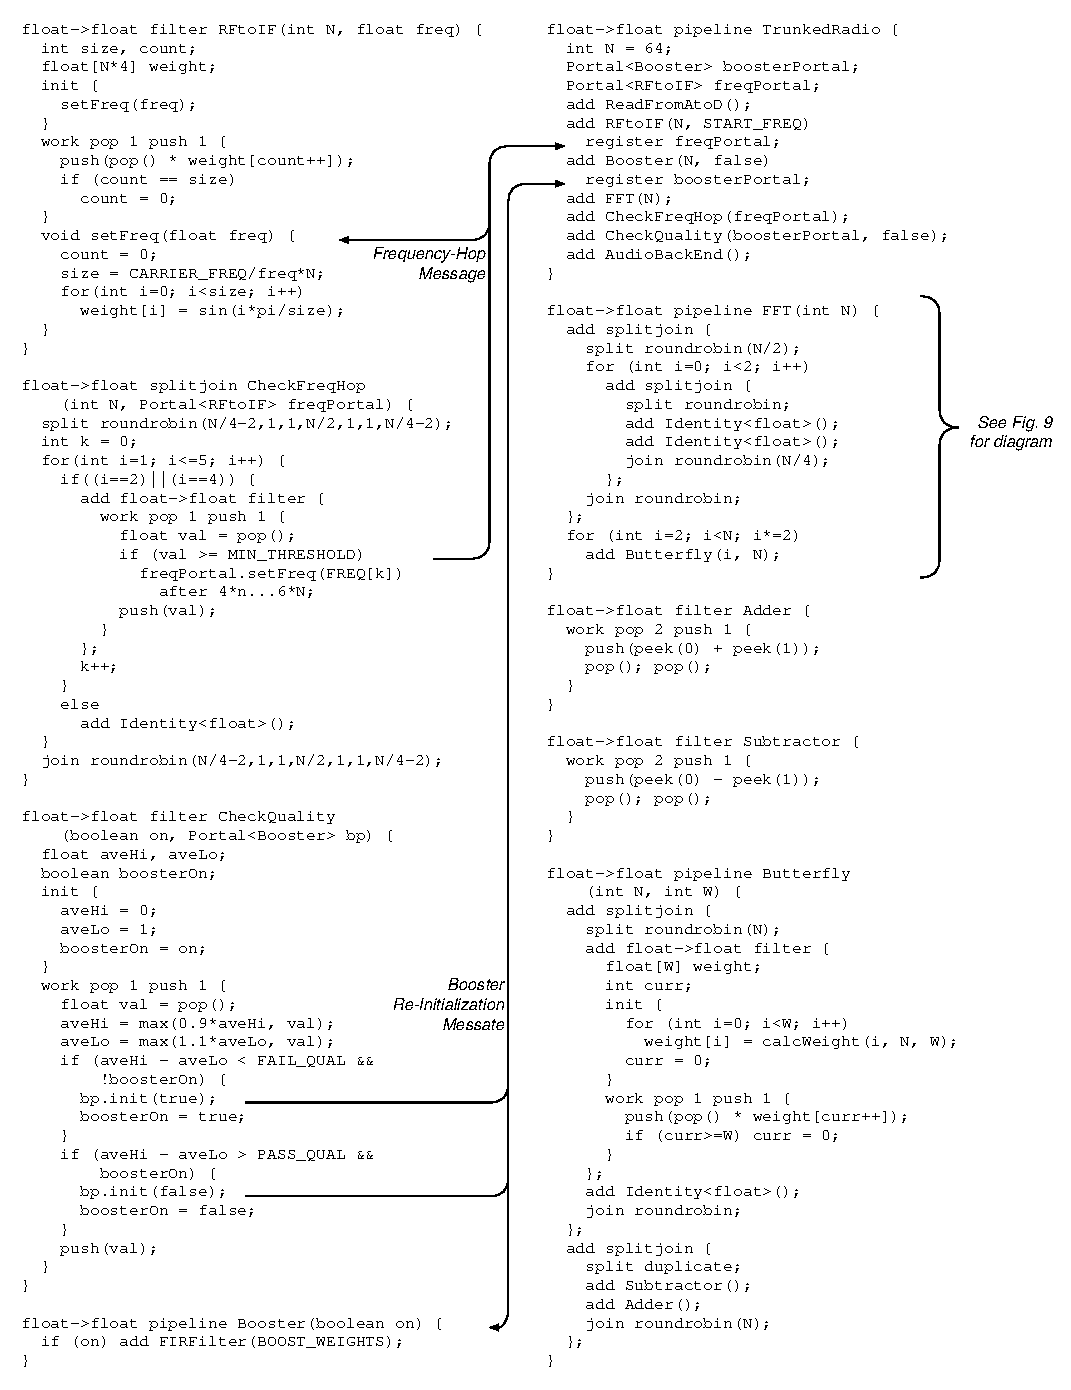
\includegraphics[width=\textwidth]{code-fm.eps}
\caption{StreamIt code for a software radio.  Arrows denote the paths
  of messages.}
\label{fig:radiocode}
\end{figure*}

We now discuss the StreamIt implementation of the Trunked Radio
illustrated in Fig.~\ref{fig:radiodiagram}.  The Trunked Radio is a
frequency-hopping system in which the receiver switches between a set of
known frequencies whenever it hears certain tones from the transmitter.

The toplevel class, \texttt{TrunkedRadio}, is implemented as a
seven-stage pipeline (see Fig.~\ref{fig:radiocode}).  The
\texttt{RFtoIF} stage modulates the input signal from RF to a
frequency band around the current IF frequency.  To support a change
in the IF frequency when frequency hopping occurs, the \texttt{RFtoIF}
filter contains a \texttt{setFreq} method that is invoked via a
message from the \texttt{CheckFreqHop} stage.  The message is sent
from \texttt{CheckFreqHop} with a latency range of $4N$ to $6N$, which
means that \texttt{RFtoIF} must deliver between $4N$ and $6N$ items
using the old modulation scheme before changing to the new frequency.

The optional \texttt{Booster} stage provides amplification for weak
signals, but is usually turned off to conserve power.  The
\texttt{Booster} is toggled by a re-initialization message from the
\texttt{CheckQuality} stage, which estimates the signal quality by the
shape of the frequency spectrum.  If all the frequencies have similar
amplitudes, \texttt{CheckQuality} assumes that the signal-to-noise
ratio is low and sends a message to activate the \texttt{Booster}.
This message is sent using best-effort delivery.

The \texttt{FFT} stage converts the signal from the time domain to the
frequency domain; please refer to p.~796 of \cite{clr} for a diagram
of the parallel FFT algorithm.  The StreamIt implementation consists
of a bit-reversal permutation followed by a series of
\texttt{Butterfly} stages.  The bit-reversal phase illustrates how
data can be reshuffled with just a few SplitJoin constructs (see
Fig.~\ref{fig:bitreverseorder}).  The \texttt{Butterfly}
stage--which is parameterized to allow for a compact representation of
the FFT--also employs split-joins to select groups of items for its
computation.  We believe that the StreamIt version of the FFT is clean
and intuitive, as the SplitJoin constructs expose the natural
parallelism of the algorithm.

%%% Local variables:
%%% TeX-master: "paper.tex"
%%% End:

  
\end{document}
